\chapter{SELF/DESTRUCT} 
\label{sec:selfdestruct}
\lstset{style=6502Style}

\vspace{-1.0cm}
\begin{figure}[H]
    \begin{adjustbox}{width=13.3cm,left}
      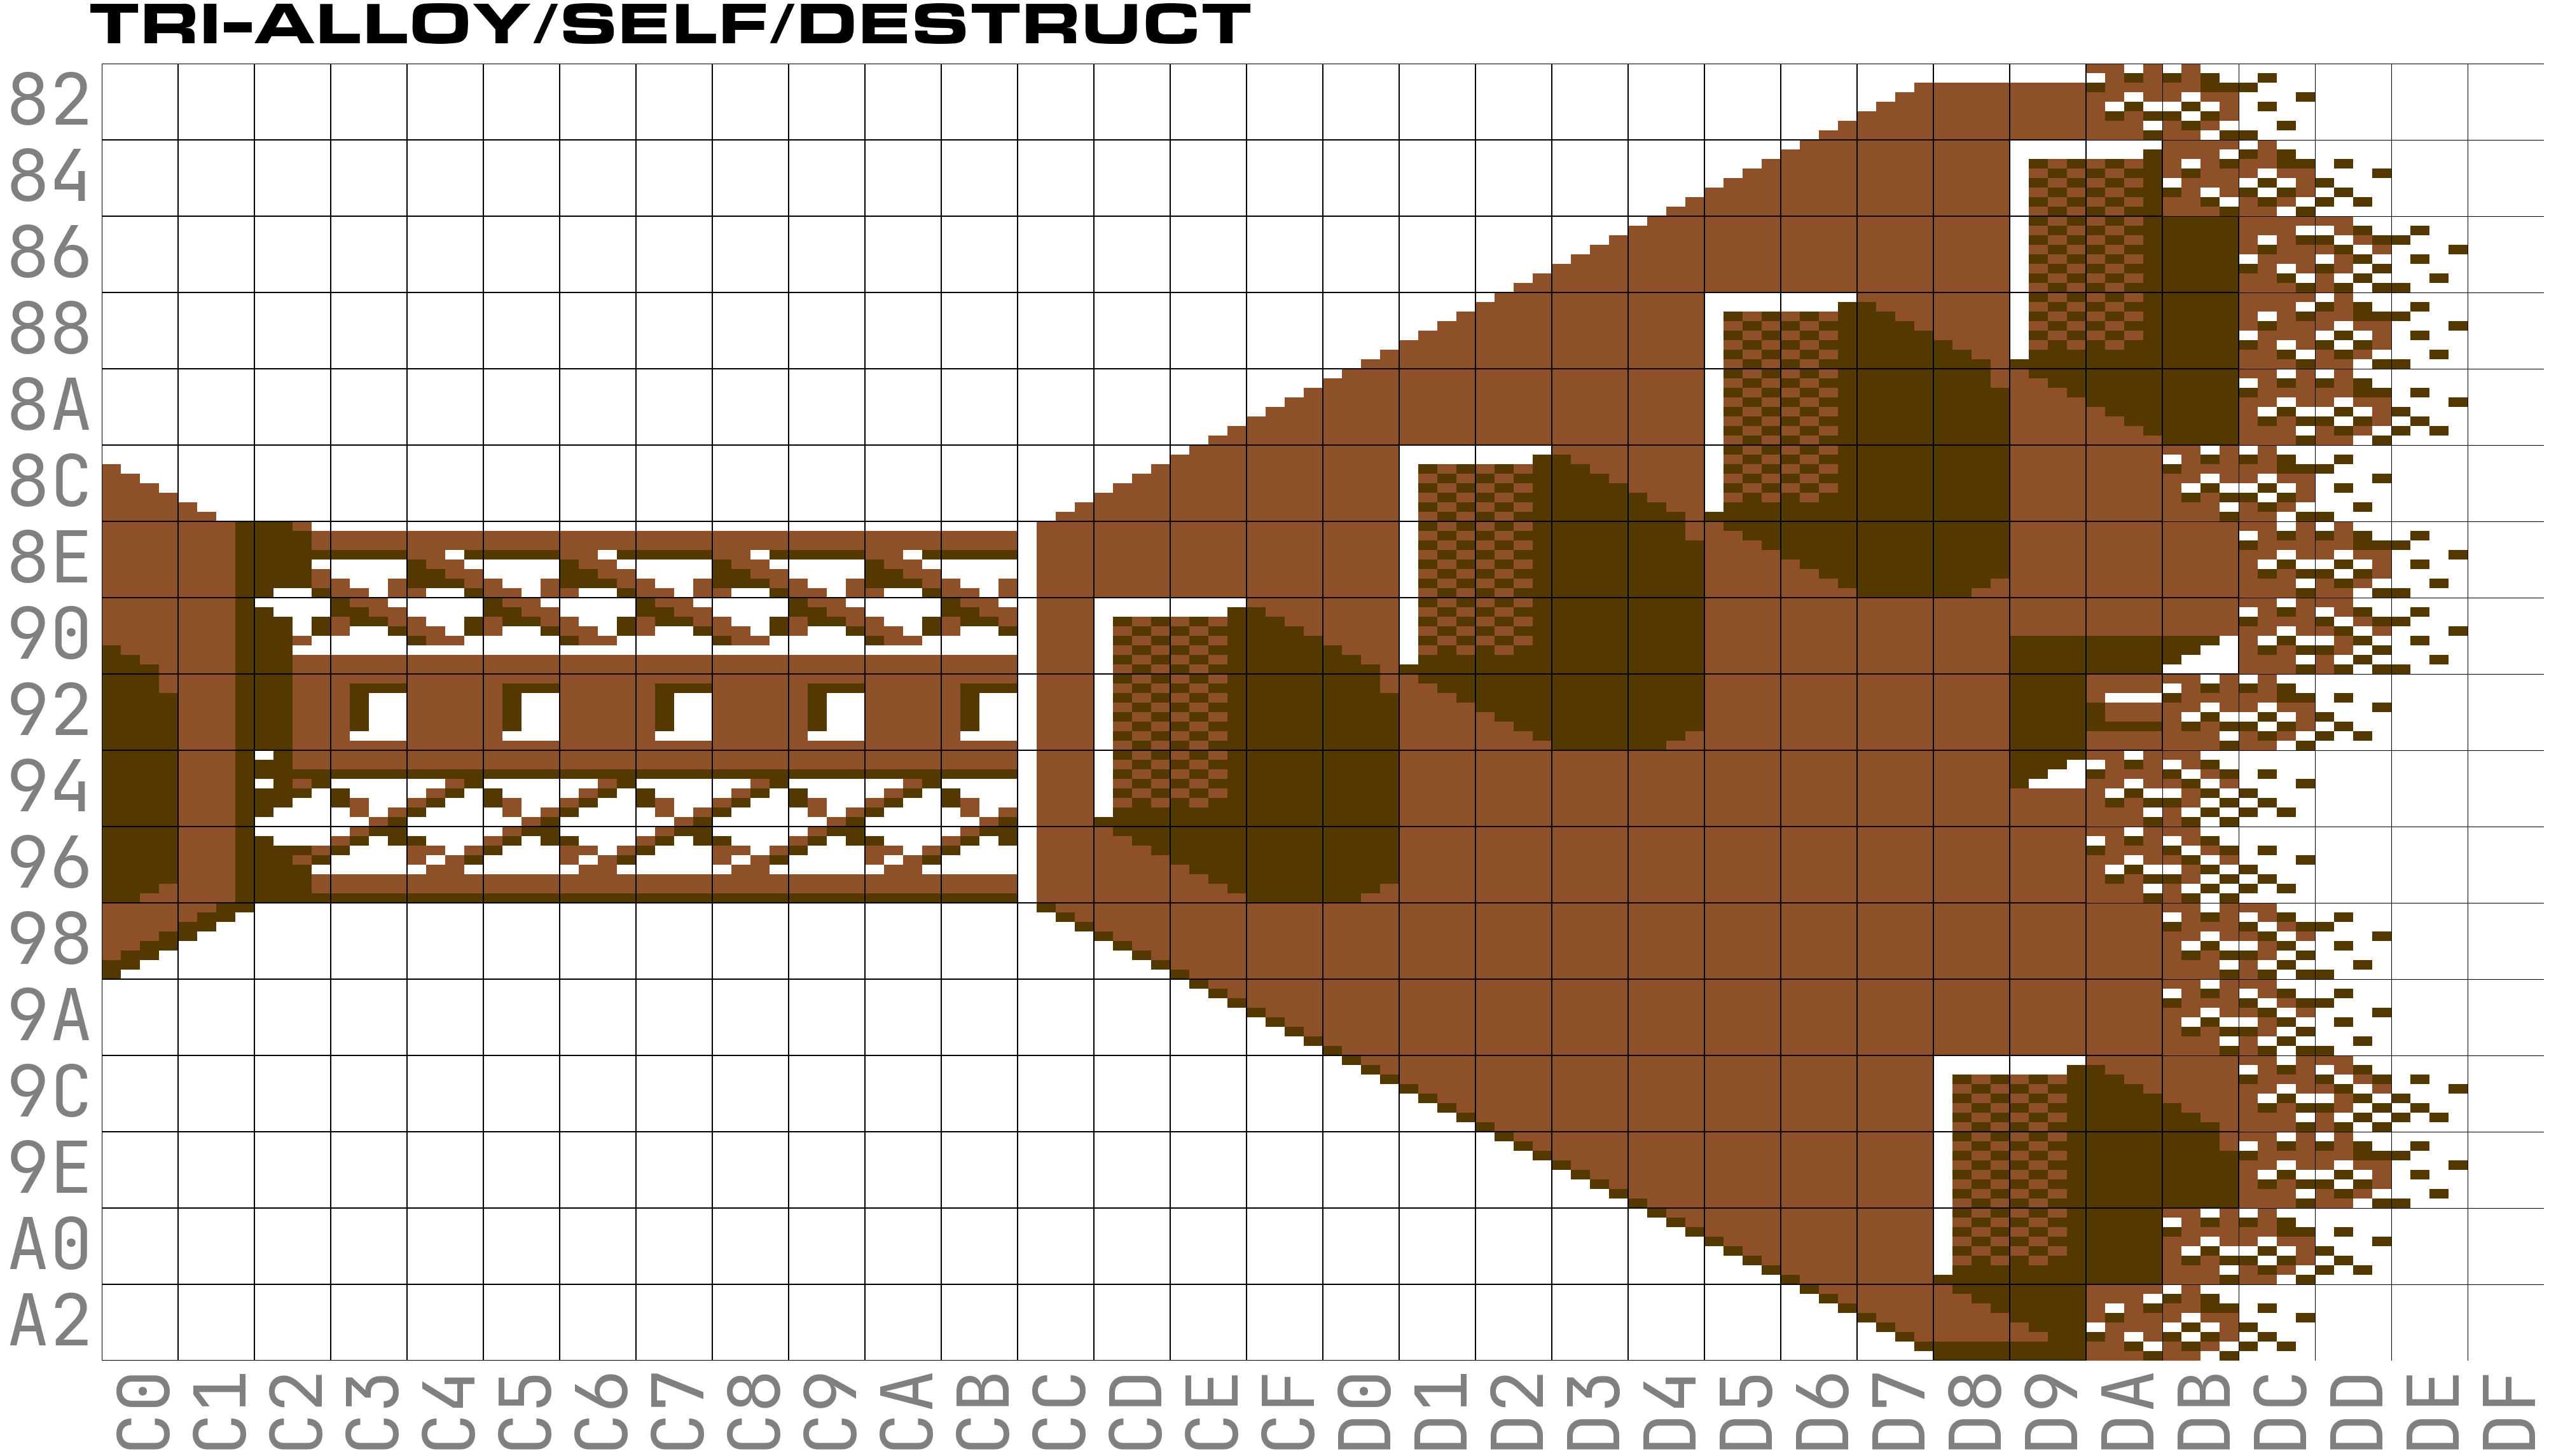
\includegraphics{src/selfdestruct/sequence/11_destruct_26_no_highlight.png}%
    \end{adjustbox}
\end{figure}
\vspace{-0.4cm}

When we complete each level, a fizzing band of destruction traverses the dreadnought obliterating
everything in its path. Close inspection reveals this band is 3 characters wide, but even looking
long and hard at the diagram above it can be hard to discern what degree of variation is at work
to give the disintegrating edge of the hull its distinctly stochastic appearance.

As it happens there are a total of six different character definitions in play, with a choice of two
for each of the three columns. These have characters \icode{F9} and \icode{FA} for the first column,
\icode{FB} and \icode{FC} for the second column, and \icode{FD} and \icode{FE} for the third.  

Putting the definitions for each side by side below gives us some idea of how they compare. Note that
the first two, which are used for the innermost of the three columns, contain disintegated ship parts.
While the second pair have just a hint of inky space provided by the two \icode{11} bit pairs. The 
definitions for the third and final column on the other hand are mostly black background, which is fitting
as they are the very edge of the destructive wave where the dreadnought is dissolving into space.

\begin{figure}[H]
    \centering
    \begin{adjustbox}{width=10cm,center}
      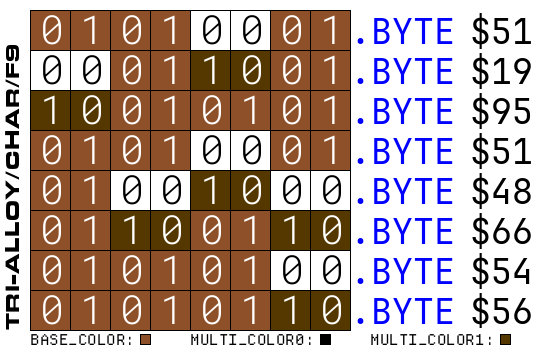
\includegraphics[width=7cm]{src/character_set_diagrams/11_F9.png}%
      \hspace{0.2cm}
      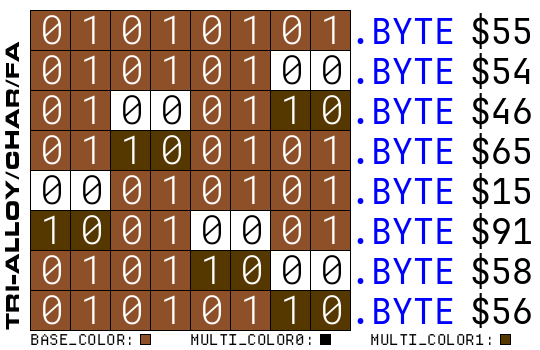
\includegraphics[width=7cm]{src/character_set_diagrams/11_FA.png}%
    \end{adjustbox}
\end{figure}
\vspace{-0.5cm}
\begin{figure}[H]
    \centering
    \begin{adjustbox}{width=10cm,center}
      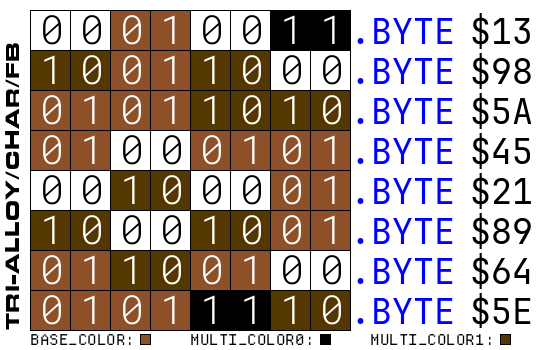
\includegraphics[width=7cm]{src/character_set_diagrams/11_FB.png}%
      \hspace{0.2cm}
      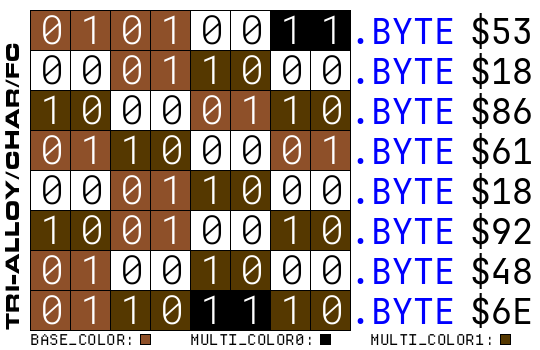
\includegraphics[width=7cm]{src/character_set_diagrams/11_FC.png}%
    \end{adjustbox}
\end{figure}
\vspace{-0.5cm}
\begin{figure}[H]
    \centering
    \begin{adjustbox}{width=10cm,center}
      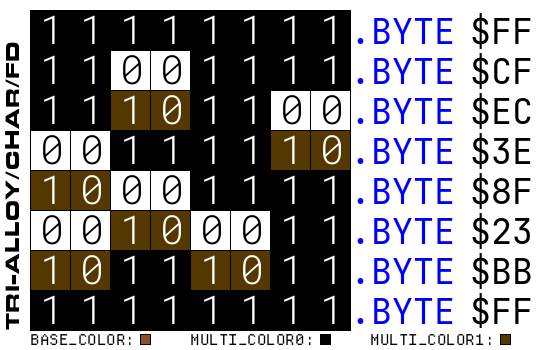
\includegraphics[width=7cm]{src/character_set_diagrams/11_FD.png}%
      \hspace{0.2cm}
      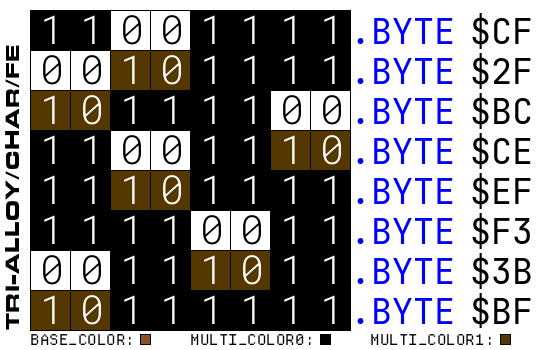
\includegraphics[width=7cm]{src/character_set_diagrams/11_FE.png}%
    \end{adjustbox}
\end{figure}
\vspace{-0.5cm}

These six characters give us a total of 8 possible permutations with which to draw the exploding
edge of the dreadnought. This is what each permutation looks like.

\begin{figure}[H]
    \centering
    \begin{adjustbox}{width=12cm,center}
      
\includegraphics[width=2cm]{src/selfdestruct/trigrams_labelled/11_F9_FB_FD.png}%
      \hspace{0.5cm}
      
\includegraphics[width=2cm]{src/selfdestruct/trigrams_labelled/11_F9_FB_FE.png}%
      \hspace{0.5cm}
      
\includegraphics[width=2cm]{src/selfdestruct/trigrams_labelled/11_F9_FC_FD.png}%
      \hspace{0.5cm}
      
\includegraphics[width=2cm]{src/selfdestruct/trigrams_labelled/11_F9_FC_FE.png}%
    \end{adjustbox}
\end{figure}
\vspace{-0.5cm}
\begin{figure}[H]
    \centering
    \begin{adjustbox}{width=12cm,center}
      
\includegraphics[width=2cm]{src/selfdestruct/trigrams_labelled/11_FA_FB_FD.png}%
      \hspace{0.5cm}
      
\includegraphics[width=2cm]{src/selfdestruct/trigrams_labelled/11_FA_FB_FE.png}%
      \hspace{0.5cm}
      
\includegraphics[width=2cm]{src/selfdestruct/trigrams_labelled/11_FA_FC_FD.png}%
      \hspace{0.5cm}
      
\includegraphics[width=2cm]{src/selfdestruct/trigrams_labelled/11_FA_FC_FE.png}%
    \end{adjustbox}
\end{figure}
\vspace{-0.5cm}

Putting them closer together gives us a better sense of how they look in practice.
\begin{figure}[H]
    \centering
    \begin{adjustbox}{width=12cm,center}
      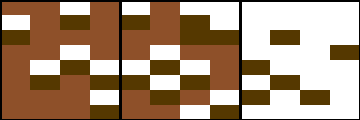
\includegraphics[width=2cm]{src/selfdestruct/trigrams_simple/11_F9_FB_FD.png}%
      \hspace{0.5cm}
      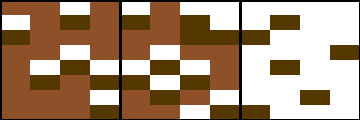
\includegraphics[width=2cm]{src/selfdestruct/trigrams_simple/11_F9_FB_FE.png}%
      \hspace{0.5cm}
      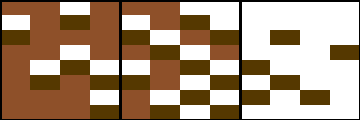
\includegraphics[width=2cm]{src/selfdestruct/trigrams_simple/11_F9_FC_FD.png}%
      \hspace{0.5cm}
      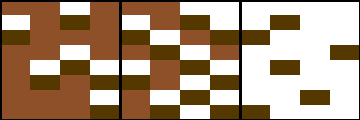
\includegraphics[width=2cm]{src/selfdestruct/trigrams_simple/11_F9_FC_FE.png}%
    \end{adjustbox}
\end{figure}
\vspace{-0.5cm}
\begin{figure}[H]
    \centering
    \begin{adjustbox}{width=12cm,center}
      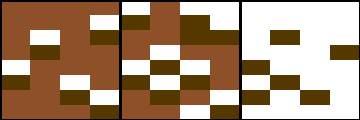
\includegraphics[width=2cm]{src/selfdestruct/trigrams_simple/11_FA_FB_FD.png}%
      \hspace{0.5cm}
      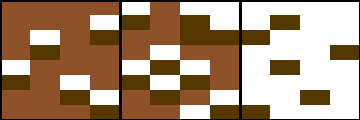
\includegraphics[width=2cm]{src/selfdestruct/trigrams_simple/11_FA_FB_FE.png}%
      \hspace{0.5cm}
      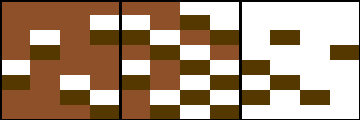
\includegraphics[width=2cm]{src/selfdestruct/trigrams_simple/11_FA_FC_FD.png}%
      \hspace{0.5cm}
      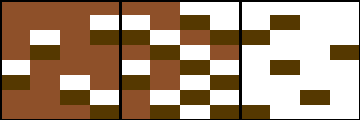
\includegraphics[width=2cm]{src/selfdestruct/trigrams_simple/11_FA_FC_FE.png}%
    \end{adjustbox}
\end{figure}
\vspace{-0.5cm}

Highlighting the band with a red grid gives us an idea of how we might go about applying
this annihilating wave to the surface of the playfield. Below we destroy 3 columns from
position \icode{DA}. We add a random offset so that the band is jagged. While the the band
is characters wide on any given line, the positions after it are erased to create empty space.

\begin{figure}[H]
    \begin{adjustbox}{width=13.3cm,left}
      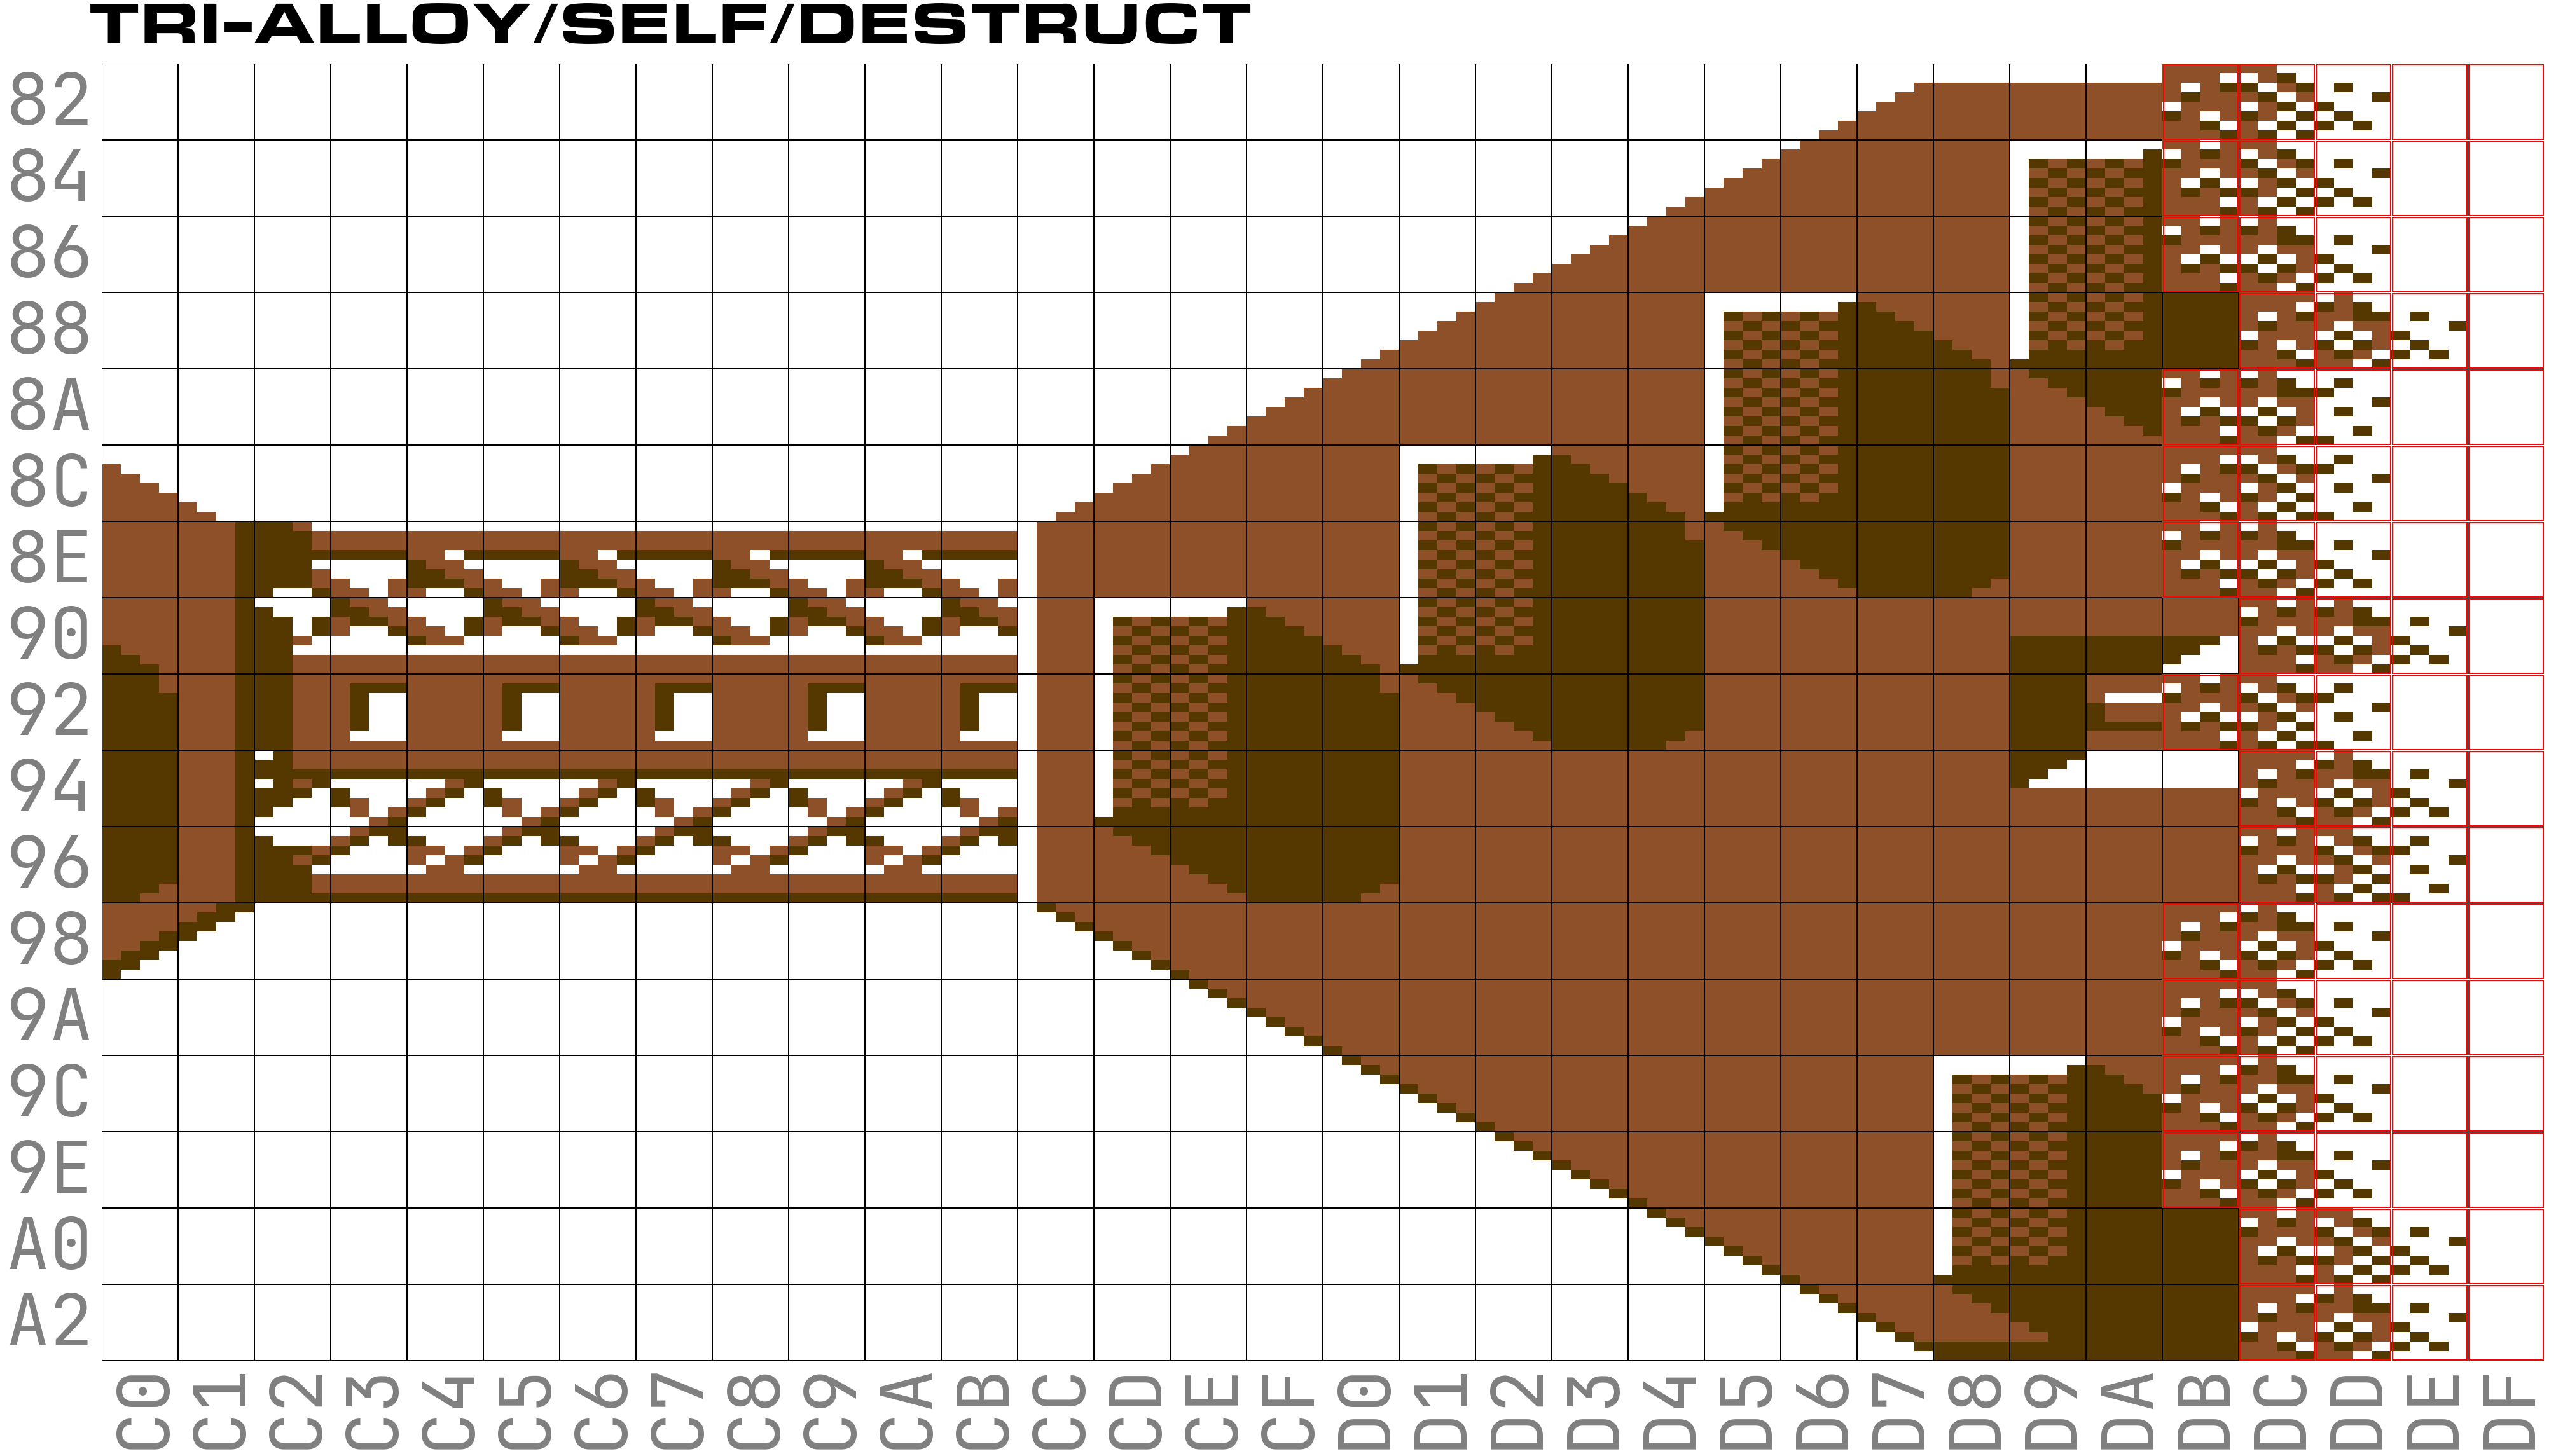
\includegraphics{src/selfdestruct/sequence/11_destruct_27.png}%
    \end{adjustbox}
\end{figure}
\vspace{-0.4cm}

In the strip below we extract the next step in the process for the three lines in the middle
of the screen.
As we advance the band across the surface we select new random permutations of the three
character configuration, though you have to look closely to notice that they are different.

\begin{figure}[H]
    \begin{adjustbox}{width=13.3cm,left}
      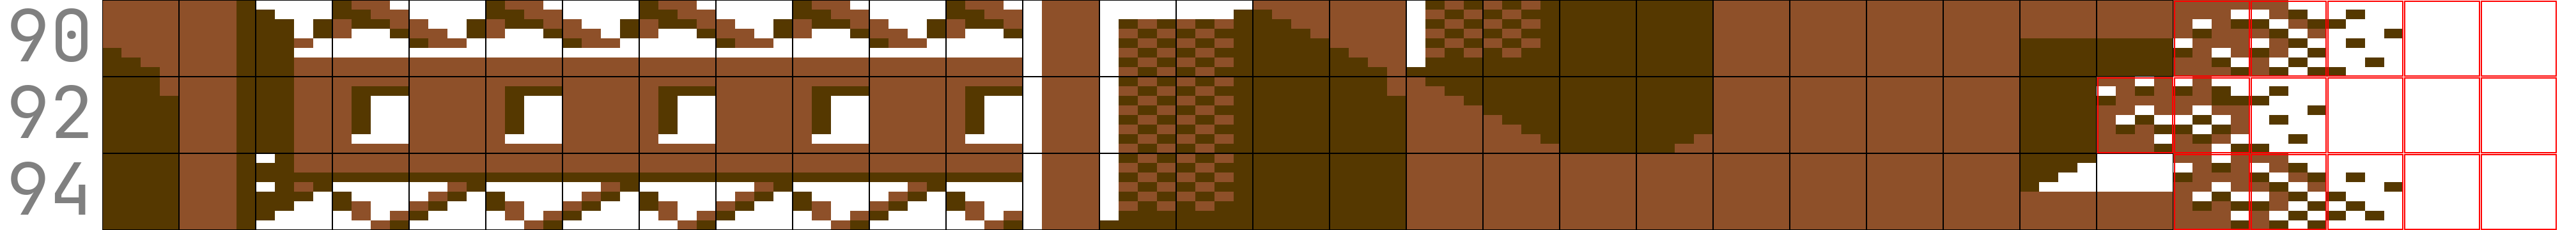
\includegraphics{src/selfdestruct/sequence/11_destruct_26_clip.png}%
    \end{adjustbox}
\end{figure}
\vspace{-0.4cm}

Advancing another column to the left we do the same. While the shape of our jagged edge
remains the same, the underlying detail mutates subtly to create a fizzing effect.
\clearpage
Notice how as we advance we fill out the columns to the right with space. There is nothing
left in the wake of our three column-wide destruction.
\begin{figure}[H]
    \begin{adjustbox}{width=13.3cm,left}
      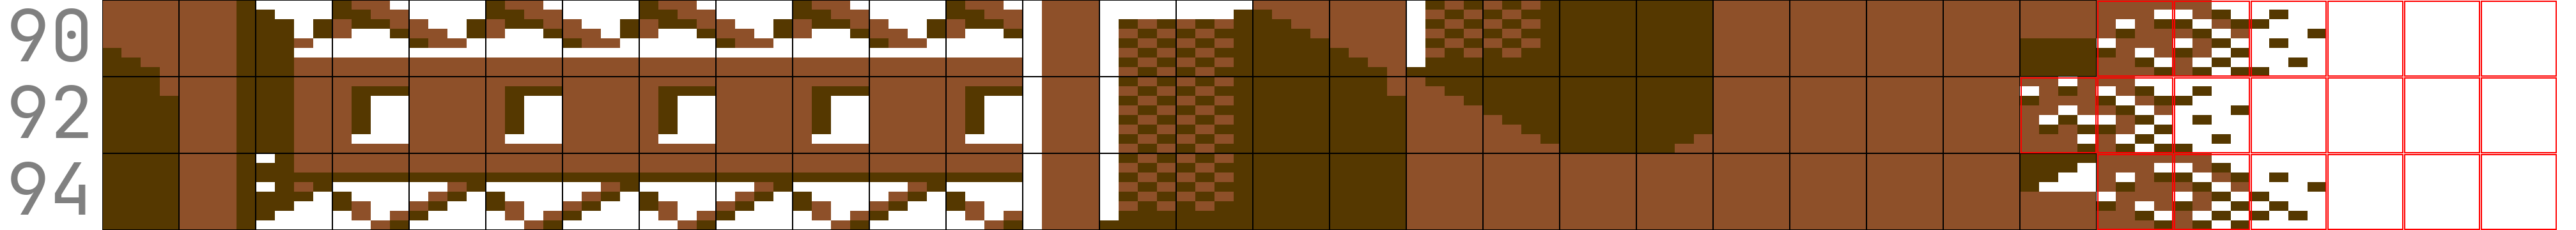
\includegraphics{src/selfdestruct/sequence/11_destruct_25_clip.png}%
    \end{adjustbox}
\end{figure}
\vspace{-0.4cm}

\begin{figure}[H]
    \begin{adjustbox}{width=13.3cm,left}
      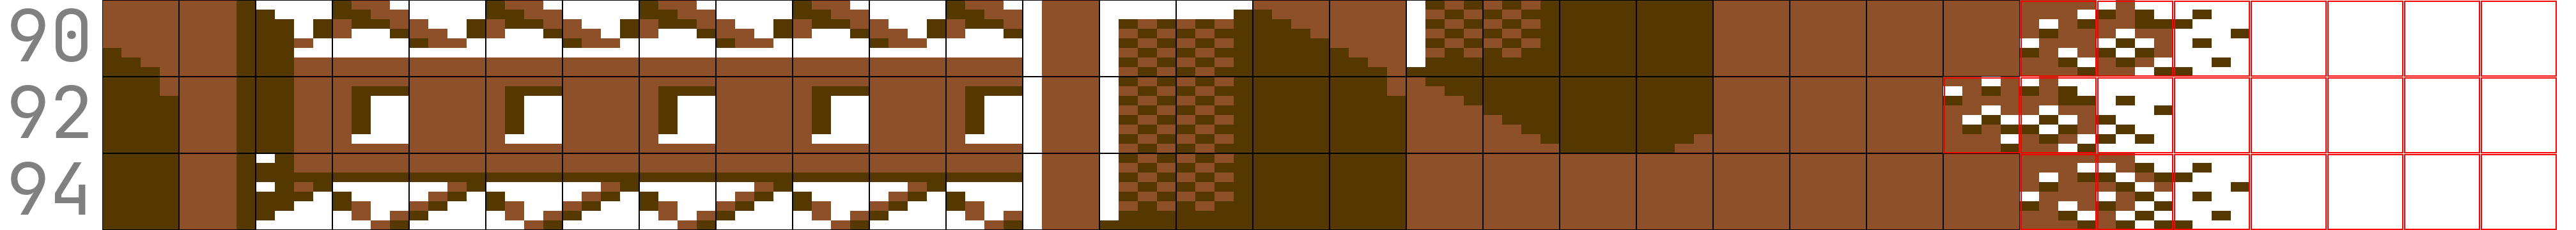
\includegraphics{src/selfdestruct/sequence/11_destruct_24_clip.png}%
    \end{adjustbox}
\end{figure}
\vspace{-0.4cm}

\begin{figure}[H]
    \begin{adjustbox}{width=13.3cm,left}
      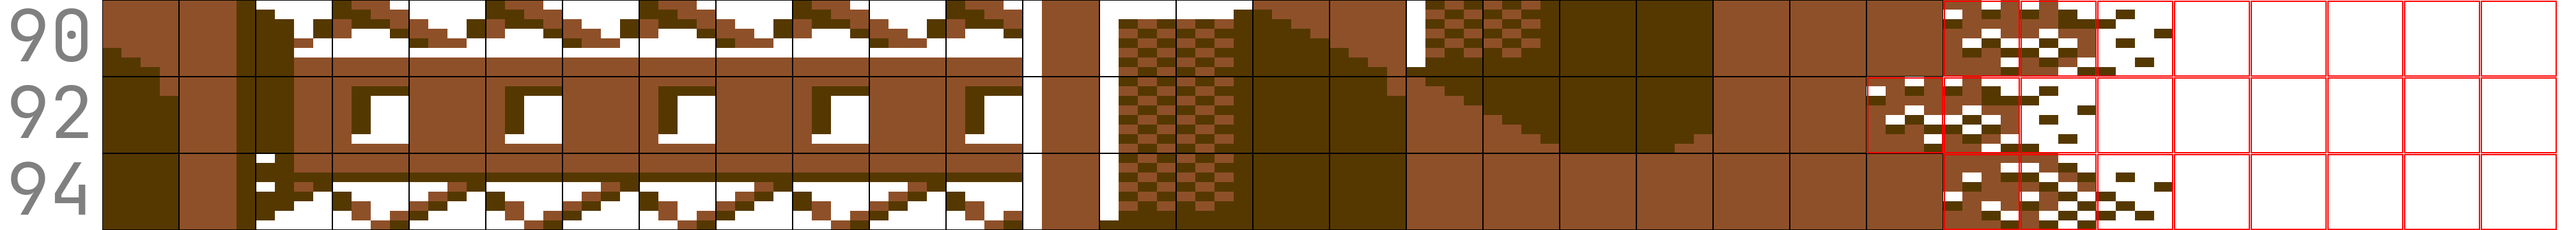
\includegraphics{src/selfdestruct/sequence/11_destruct_23_clip.png}%
    \end{adjustbox}
\end{figure}
\vspace{-0.4cm}

\begin{figure}[H]
    \begin{adjustbox}{width=13.3cm,left}
      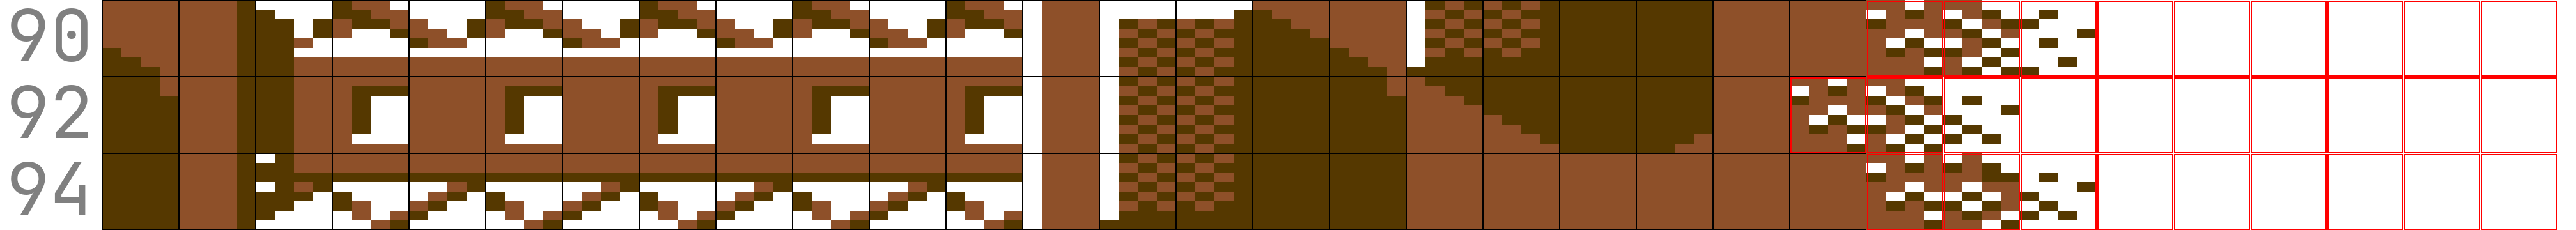
\includegraphics{src/selfdestruct/sequence/11_destruct_22_clip.png}%
    \end{adjustbox}
\end{figure}
\vspace{-0.4cm}

The routine that implements this process is given below,
\icode{DisintegrateDreadnought}. Each time it's called it draws the edge of
destruction across the current position on the surface and then advances its pointers
to the next position in wait for the next time it's invoked.
Notice how the routine is careful to avoid destroying empty space. For each of the
three characters that we're going to destroy we first detect if they are empty space. If they
are, we skip to the next character. This avoids the displeasing possibility of appearing to 
add destroyed debris to the empty background. 
Notice also how we avoid unnecessary work at the start of the routine by ensuring we're in
a section of the playfield that actually contains some dreadnought to destroy: if we're in a segment
that is completely blank such as at the start or end of the map we exit the routine early without doing anything at all.

\begin{lstlisting}
DisintegrateDreadnought
  ; Our current 'edge of destruction' is stored in 
  ; destroyedEdgeLoPtr/destroyedEdgeHiPtr. We move this edge
  ; one column to the left across the dreadnought with each visit
  ; to this routine.
  LDA destroyedEdgeLoPtr     ; Get low byte of current edge.
  STA surfaceDataLoPtr       ; Store in surfaceDataLoPtr.
  LDA destroyedEdgeHiPtr     ; Get high byte of current edge.
  STA surfaceDataLoPtr       ; Store in surfaceDataLoPtr.
  CMP #$82                   ; Are we in the first half of the surface yet?
  BNE DestroyCurrentEdge     ; If not, find some surface to destroy.
  LDA destroyedEdgeLoPtr     ; If we're in the first half..
  CMP #SPACE                 ; .. check for empty space, and..
  BCC Skip                   ; .. if empty, just return early.
\end{lstlisting}
\begin{lstlisting}
  ; Destroy a full edge with 3 columns of 'destroyed' dreadnought, and
  ; write empty space to the 3 columns after that.
DestroyCurrentEdge
  LDX #17                    ; Loop for all 17 rows of the dreadnought.

DestroyARow
DestroyColumn1  
  LDY jaggedEdgePositions,X  ; Get the offset to use for a jagged effect.
  LDA (surfaceDataLoPtr),Y   ; Get the character for the current row.
  CMP #SPACE                 ; Is it empty space?
  BEQ DestroyColumn2         ; If so, we don't need to destroy it.
  LDA $D41B                  ; Get a random number.
  AND #$01                   ; Make it a random number between 0 and 1.
  ADC #$F9                   ; Add it to $F9, so we have $F9 or $FA.
  STA (surfaceDataLoPtr),Y   ; Use that as the 'damage' character.

DestroyColumn2  
  INY                        ; Go to the next column.
  LDA (surfaceDataLoPtr),Y   ; Get the character for the current row.
  CMP #SPACE                 ; Is it empty space?
  BEQ DestroyColumn3         ; If so, we don't need to destroy it.
  LDA $D41B                  ; Get a random number.
  AND #$01                   ; Make it a random number between 0 and 1.
  ADC #$FB                   ; Add it to $FB, so we have $FB or $FC.
  STA (surfaceDataLoPtr),Y ; Use that as the 'damage' character. 

DestroyColumn3  
  INY                        ; Go the next column.
  LDA (surfaceDataLoPtr),Y   ; Get the character for the current row.
  CMP #SPACE                 ; Is it empty space?
  BEQ EraseLast3Cols         ; If so, we don't need to destroy it.
  LDA $D41B                  ; Get a random number.
  AND #$01                   ; Make it a random number between 0 and 1.
  ADC #$FD                   ; Add it to $FD, so we have $FD or $FE.
  STA (surfaceDataLoPtr),Y ; Use that as the 'damage' character. 

  ; Now that we've destroyed an edge with 3 columns of 'destruction'
  ; make sure that we create 3 columns of empty space in our wake.
EraseLast3Cols
  INY                        ; Go to the next column.
  LDA #SPACE                 ; Load a space character to A.
  STA (surfaceDataLoPtr),Y   ; Write empty space to the surface.
  INY                        ; Go to the next column.
  STA (surfaceDataLoPtr),Y   ; Write empty space to the surface.
  INY                        ; Go to the next column.
  STA (surfaceDataLoPtr),Y   ; Write empty space to the surface.

  INC surfaceDataLoPtr       ; Move to the next row in the surface data..
  INC surfaceDataLoPtr       ; e.g. from $8200 to $8400.
  DEX                        ; Move to the next row.
  BNE DestroyARow            ; Keep going until all rows are done.
\end{lstlisting}
\clearpage
\begin{lstlisting}
  ; Move our edge one column further along the dreadnought 
  ; for the next time that we're called.
  LDA destroyedEdgeLoPtr     ; Get the current edge address.
  SBC #$01                   ; Subtract by one.
  STA destroyedEdgeLoPtr     ; Update the current edge.
  LDA destroyedEdgeHiPtr     ; Update the high byte of the address..
  SBC #$00                   ; if necessary by applying the carry but.
  STA destroyedEdgeHiPtr

Skip
  RTS                        ; We're done destroying the column.
\end{lstlisting}

With this we can advance the wave inexorably, calling \icode{DisintegrateDreadnought}
as we scroll across the screen, eating up the surface below.

\begin{figure}[H]
    \begin{adjustbox}{width=13.3cm,left}
      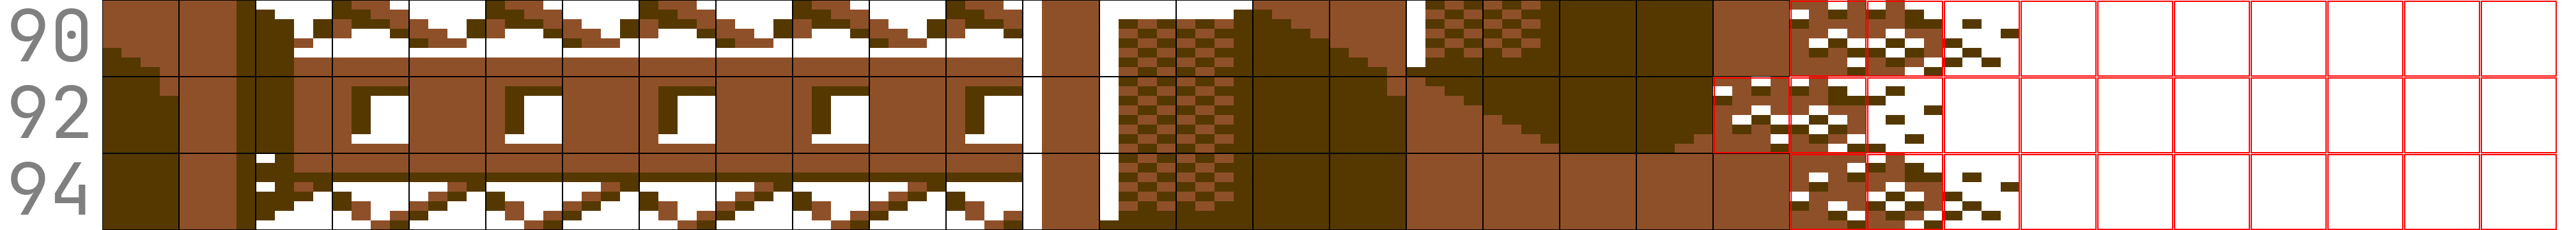
\includegraphics{src/selfdestruct/sequence/11_destruct_21_clip.png}%
    \end{adjustbox}
\end{figure}
\vspace{-0.4cm}

\begin{figure}[H]
    \begin{adjustbox}{width=13.3cm,left}
      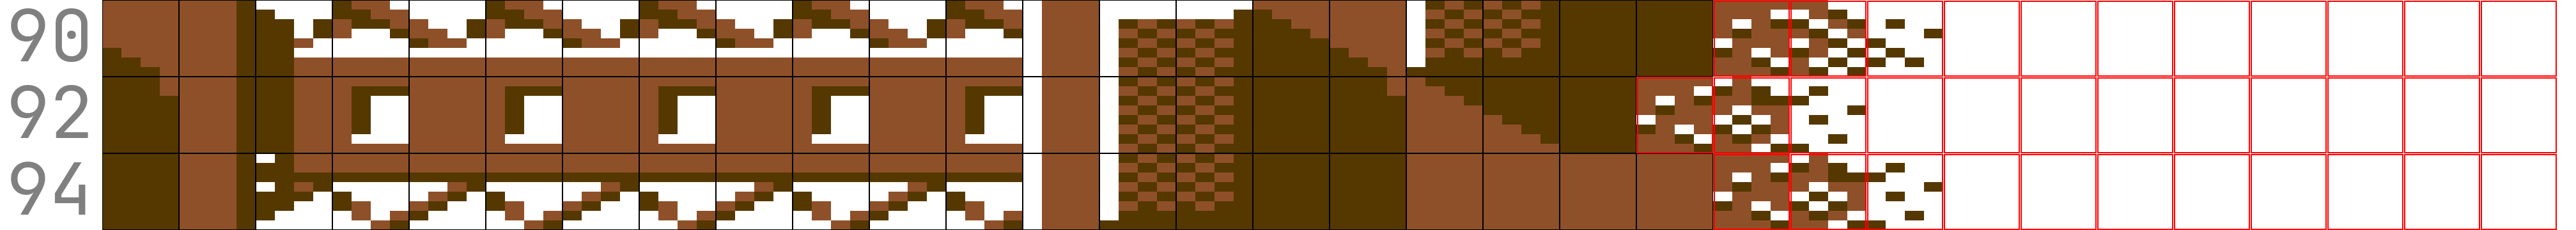
\includegraphics{src/selfdestruct/sequence/11_destruct_20_clip.png}%
    \end{adjustbox}
\end{figure}
\vspace{-0.4cm}

\begin{figure}[H]
    \begin{adjustbox}{width=13.3cm,left}
      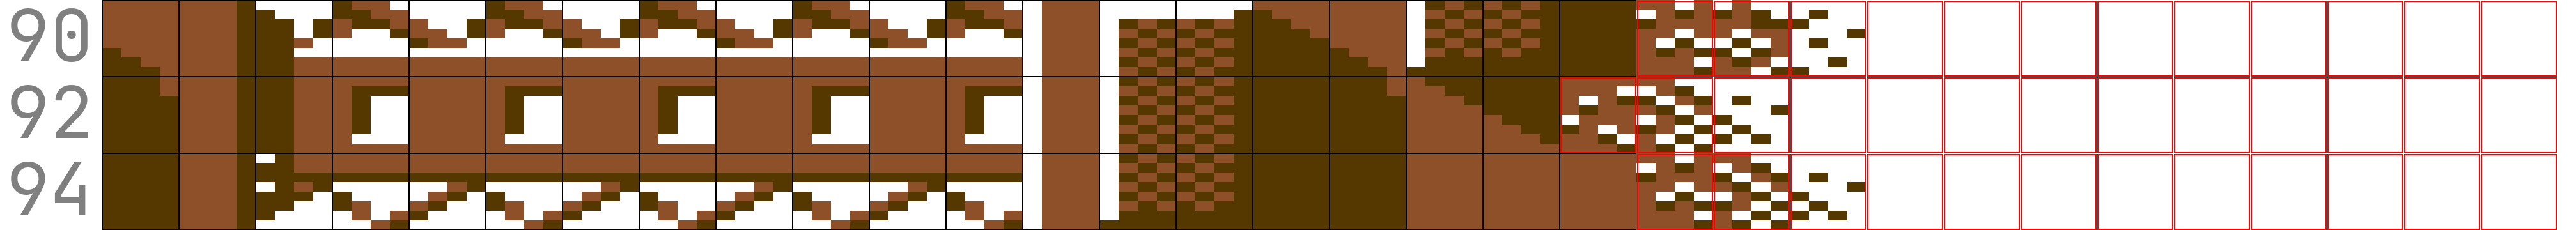
\includegraphics{src/selfdestruct/sequence/11_destruct_19_clip.png}%
    \end{adjustbox}
\end{figure}
\vspace{-0.4cm}

\begin{figure}[H]
    \begin{adjustbox}{width=13.3cm,left}
      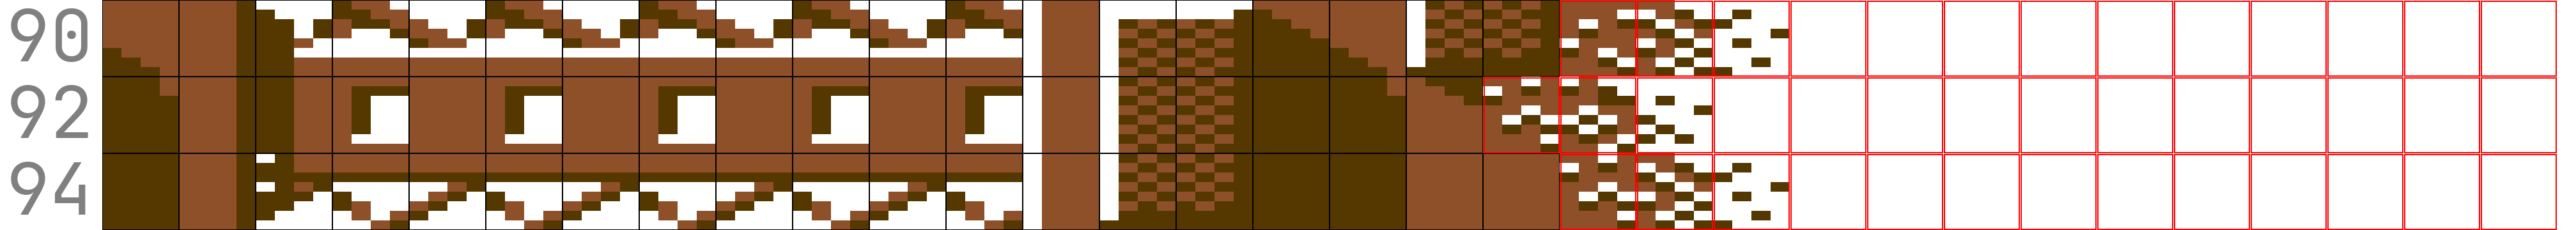
\includegraphics{src/selfdestruct/sequence/11_destruct_18_clip.png}%
    \end{adjustbox}
\end{figure}
\vspace{-0.4cm}
